\chapter{Overview of the Implementation}

In the previous chapters we looked at the design and implementation of the different system part there are in the Media-Online Management (MOM).
In this chapter we are going to show how it all of the parts are working together.

In figure \ref{fig:deployment} is a deployment and component diagram of the Media-Online Management system. There are a tag-reader and an Arduino node this is the controller. The controller is working independently of the website but it is dependent on the API. In the future if the Arduino should be replaced or another type of controller also should be used with MOM then it is only the code on the controller which should be adapted. 
On the centralized server there are five components: the Website, API, Daemon, Function lib, and the Database. All dependencies of among the components is going downwards from a system and user interfaces to the functions lib which manipulate the data in the database which is independent of all the components.
 The components Website, API and Daemon can be replaced without changing anything further in the system. However, if the component is API it could affect the controller if the system interface does not remain the same.
    
\begin{figure}
	\centering
		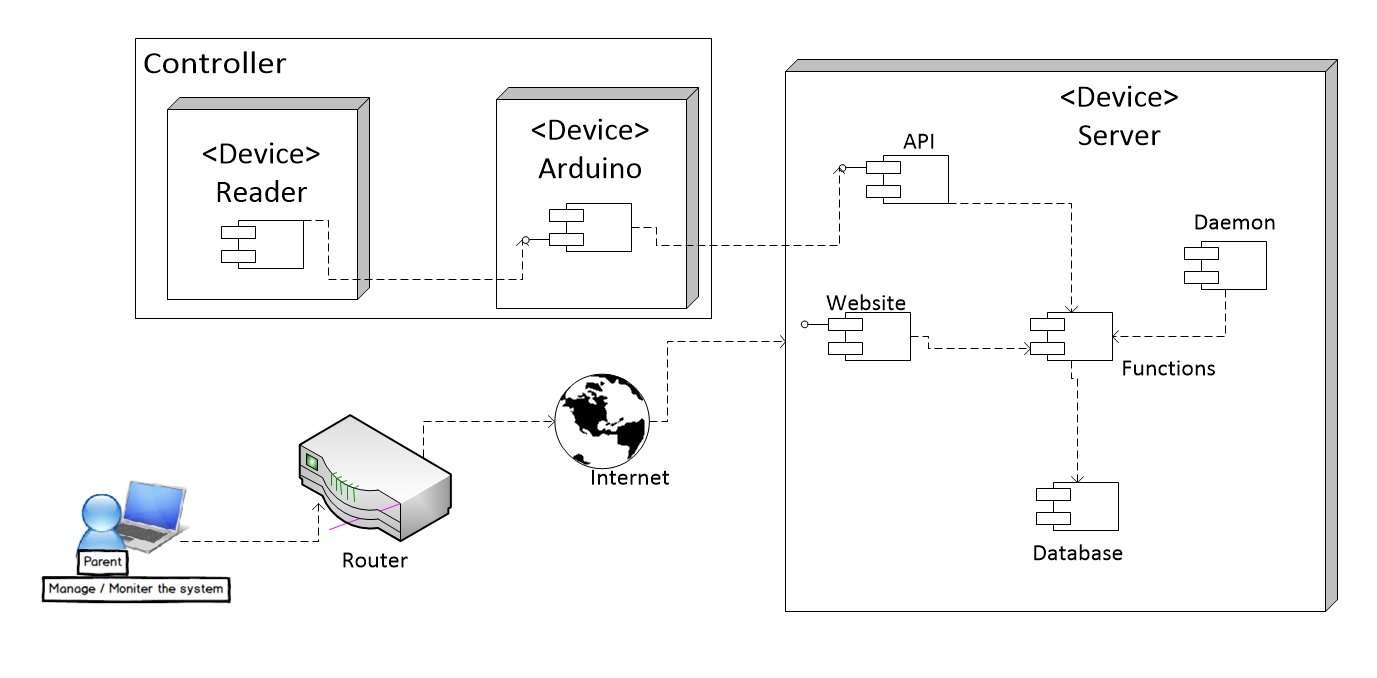
\includegraphics[width=1.50\textwidth, angle=90 ]{images/deployment.jpg}
	\caption{Deployment and component diagram}
	\label{fig:deployment}
\end{figure}



Before going explaining the testing of MOM, we are going to summarize some of the conclusion that the previous chapters came to.

\subsection*{The Database and the function library}
The database is able to store all relevant data that are to be used by different system parts. In the database rule's and permission's data is considered to be the same. The tables that are storing a conditions data uses partitioning to avoid redundancy and reduce null values. In the database we use DELETE CASCADE with all foreign keys which mean that when a object is deleted then all of the references to this object is deleted.

The function library consist of several functions that are able to manipulate the data in the database. The database and many of the functions support that a rule can have several actions and conditions, but some of the functions only support one condition and action.
 
\subsection*{The API}
\subsection*{The Daemon}
\subsection*{The Website}
\subsection*{The Arduino}
The Arduino is the implemented solution for controlling interaction with media devices and it has been issued with both the software and extension in hardware to function in this capacity.
To turn on a device the user must swipe his tag over the RFID antenna.
Upon the swipe, the Arduino will read the Tag ID and call the API to check for permission to turn on the device, and if the permission is granted, the Arduino will do so.
The Media device will continue to run until one of three events occur: The user chooses to log out from the device, which is done with another swipe and another call to the API. The user could also run out of time, at which point the Arduino shuts off the device. Finally, status updates, which the Arduino gets from calling the API regularly, could tell the Arduino to shut off.